

%%%%%%%%%%%%%%%%%%%%%%%%%%%%%%%%%%%%%%%%%%%%%%%%%%%%%%%%%%%%%%%%%%%%%%%%%%%%%%%%%%%%%%%%%%%%%
%%									ANNEXES 												%
%%%%%%%%%%%%%%%%%%%%%%%%%%%%%%%%%%%%%%%%%%%%%%%%%%%%%%%%%%%%%%%%%%%%%%%%%%%%%%%%%%%%%%%%%%%%%
\chapter{Annexes} \label{Annexes}

%%%%%%%%%%%%%%%%%%%%%%%%%%%%%%%%%%%%%%%%%%%%%%%%%%%%%%%%%%%%%%%%%%%%%%%%%%%%%%%%%%%%%%%%%%%%%


\section*{Figures annexes}

\begin{figureth}
	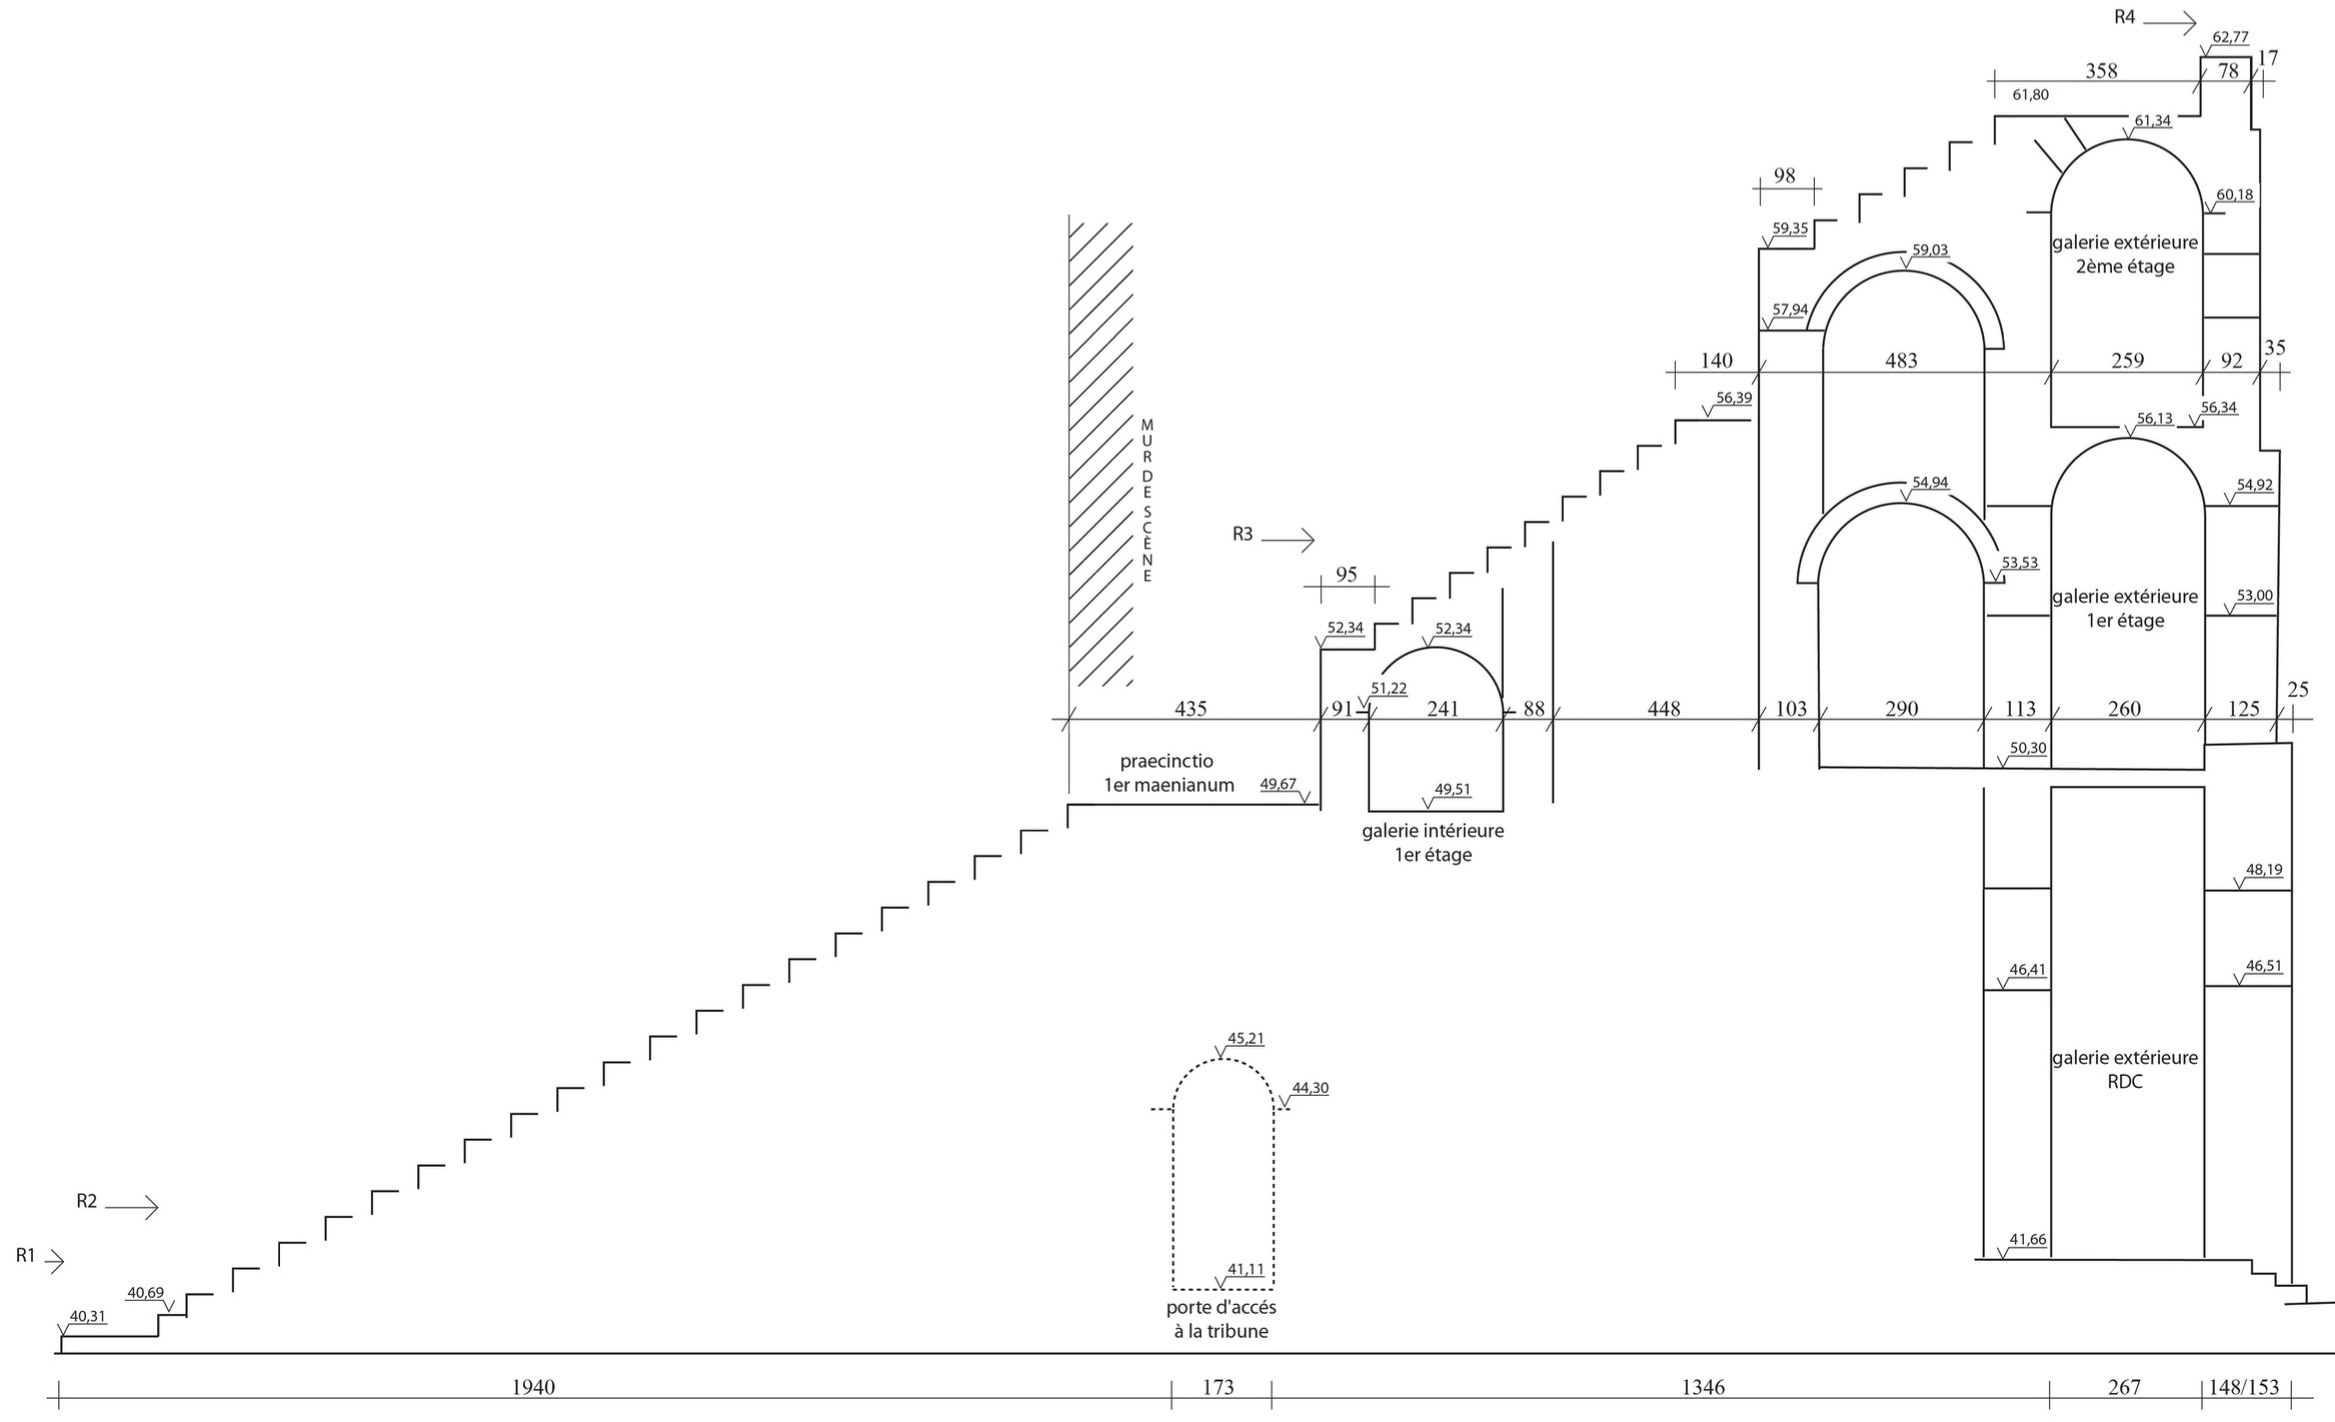
\includegraphics[width=\linewidth]{images/CoupeCavea}
	\caption[Coupe théorique sur la \gls{cavea}.]{Coupe théorique sur la \gls{cavea} \cite[Pl. LX]{orangePl}.} 
	\label{coupeCavea} 
\end{figureth}

\begin{figureth}
	\includegraphics[width=\linewidth]{images/caristieDessus}
	\caption[Vue de dessus par A. Caristie 1856.]{Représentation de l'état du théâtre d'Orange en 1856 en vue de dessus par A. Caristie \cite[Pl. I]{orangePl}.} 
	\label{caristieDessus} 
\end{figureth}
	
\begin{figureth}
	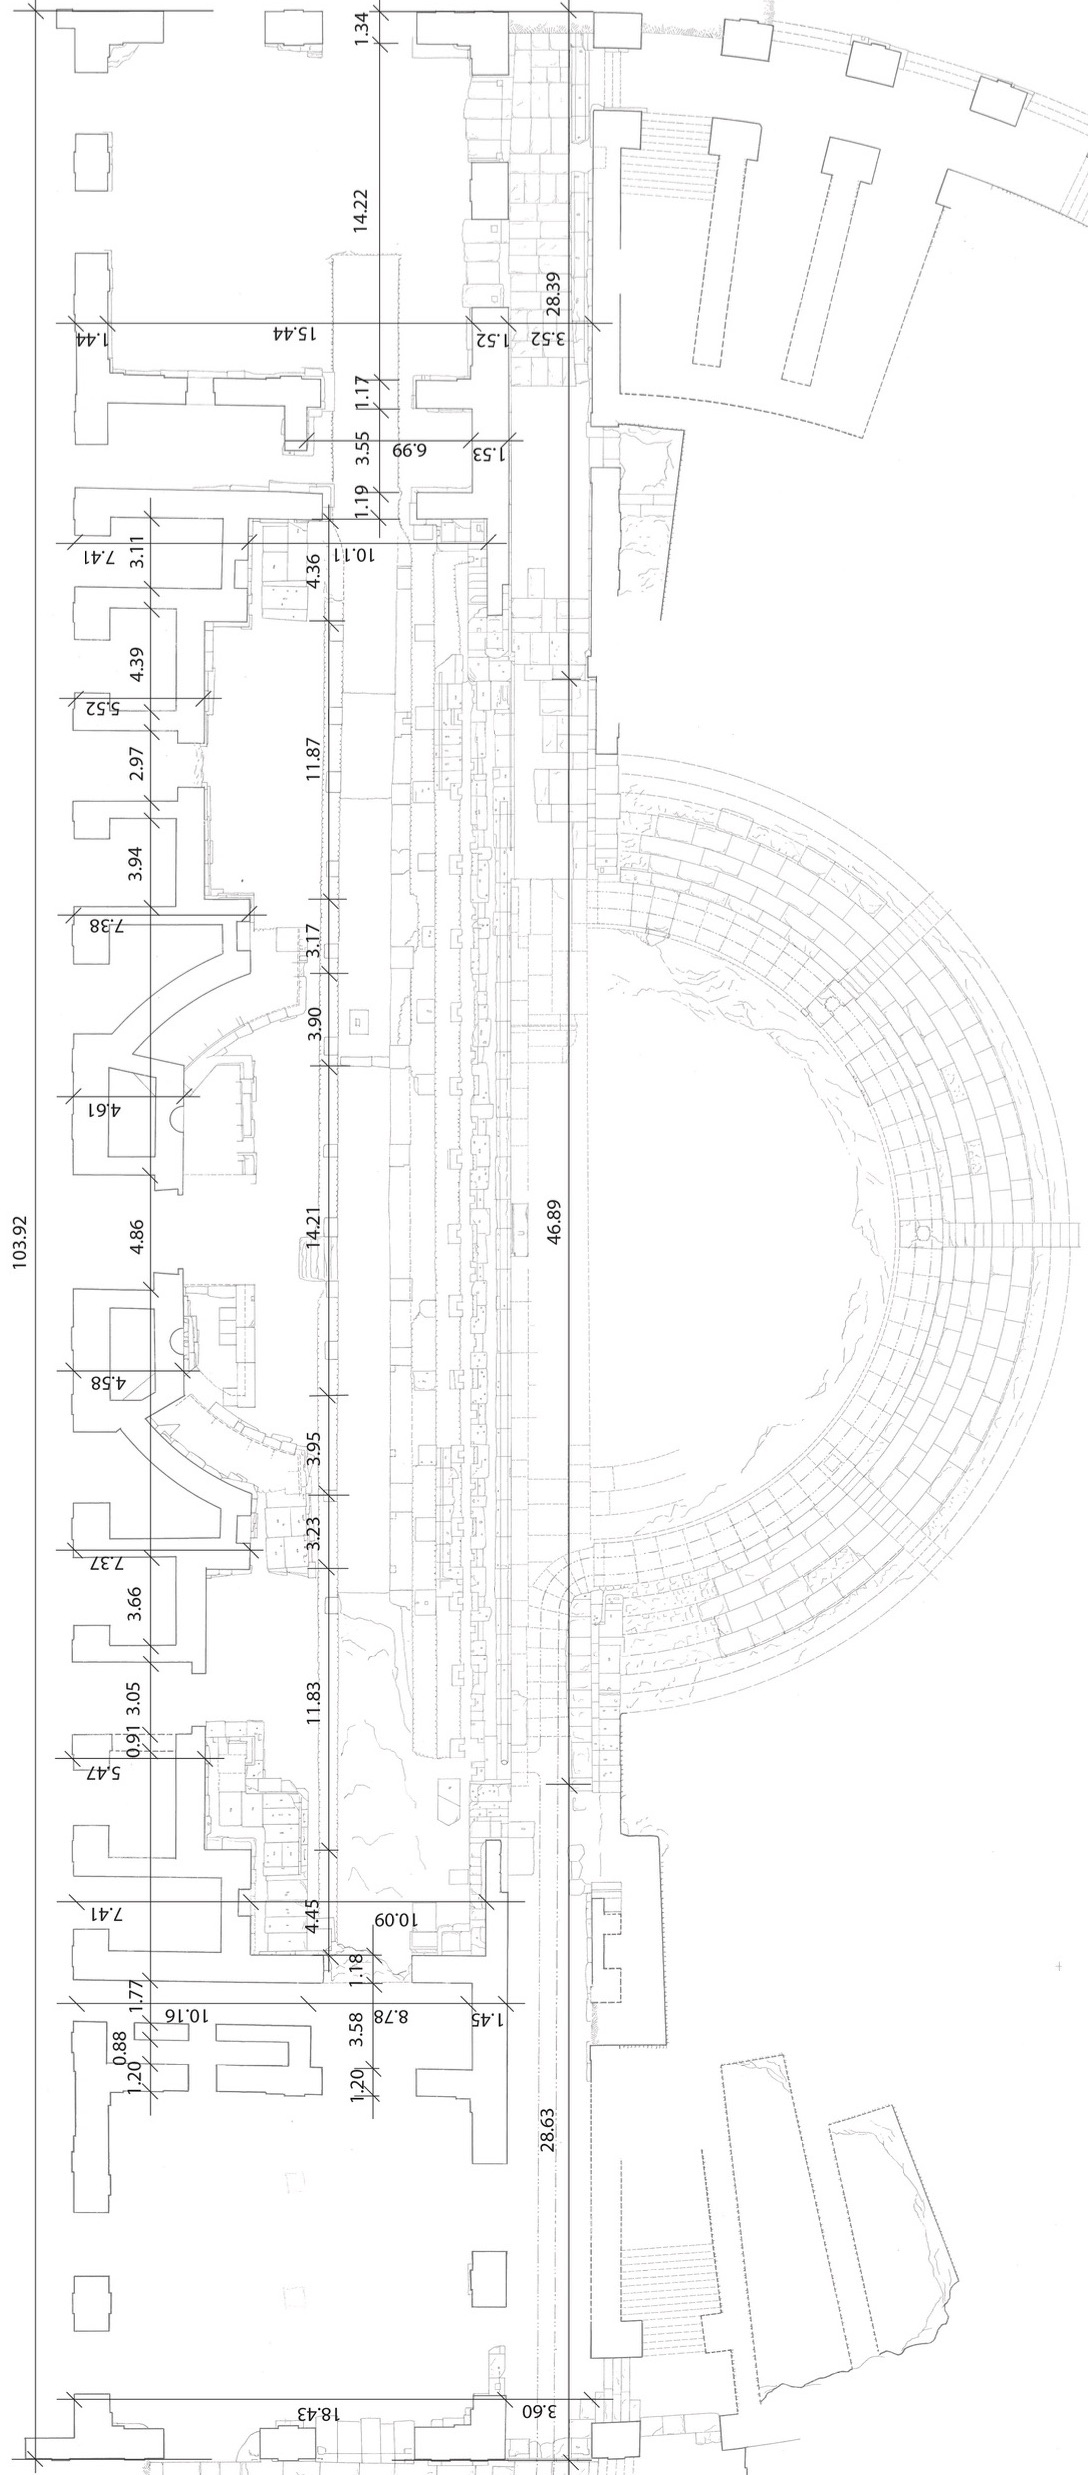
\includegraphics[height=0.8\paperheight]{images/cotes}
	\caption[Plan du rez-de-chaussée au bâtiment de scène.]{Plan du rez-de-chaussée au bâtiment de scène \cite[Pl. XXI]{orangePl}.}
	\label{cotes} 
\end{figureth}

\begin{figureth}
		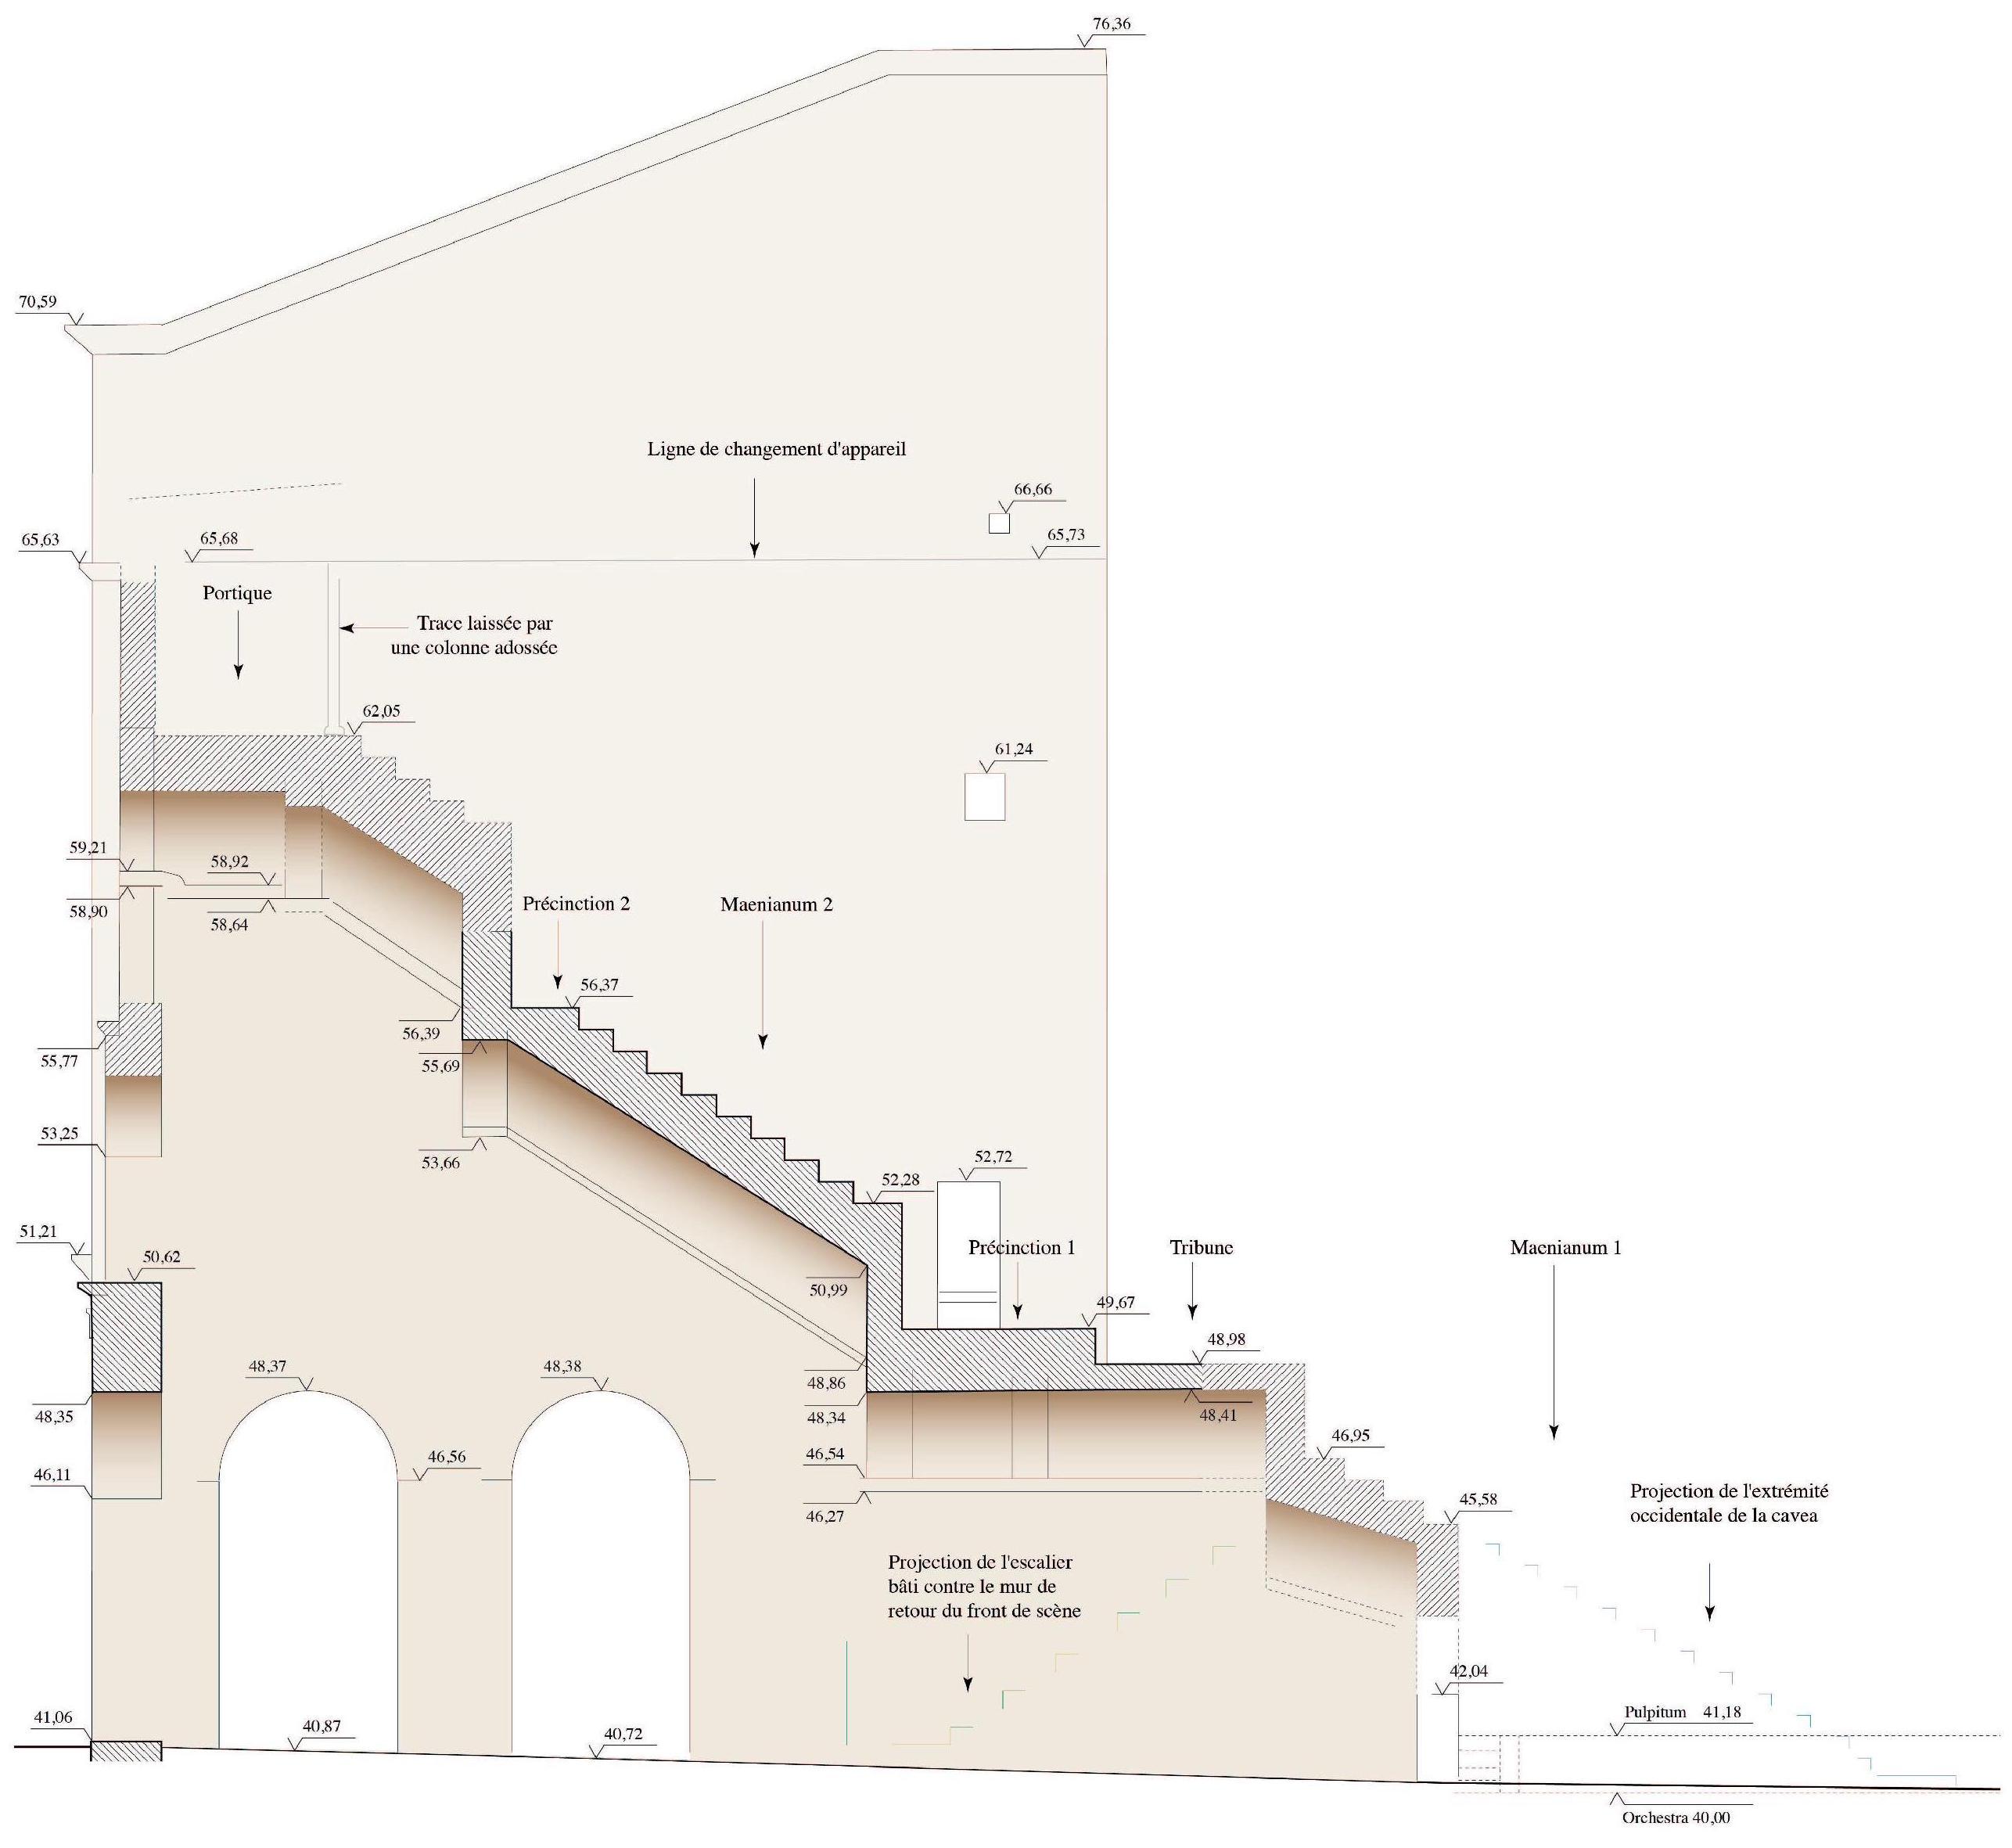
\includegraphics[width=\linewidth]{images/aditusOccidental}
		\caption[Coupe sur l'\gls{aditus} occidental]{Coupe sur l'\gls{aditus} occidental \cite[Pl. XLVIII]{orangePl}.}
		\label{aditusOccidental}	
\end{figureth}

\begin{figureth}
		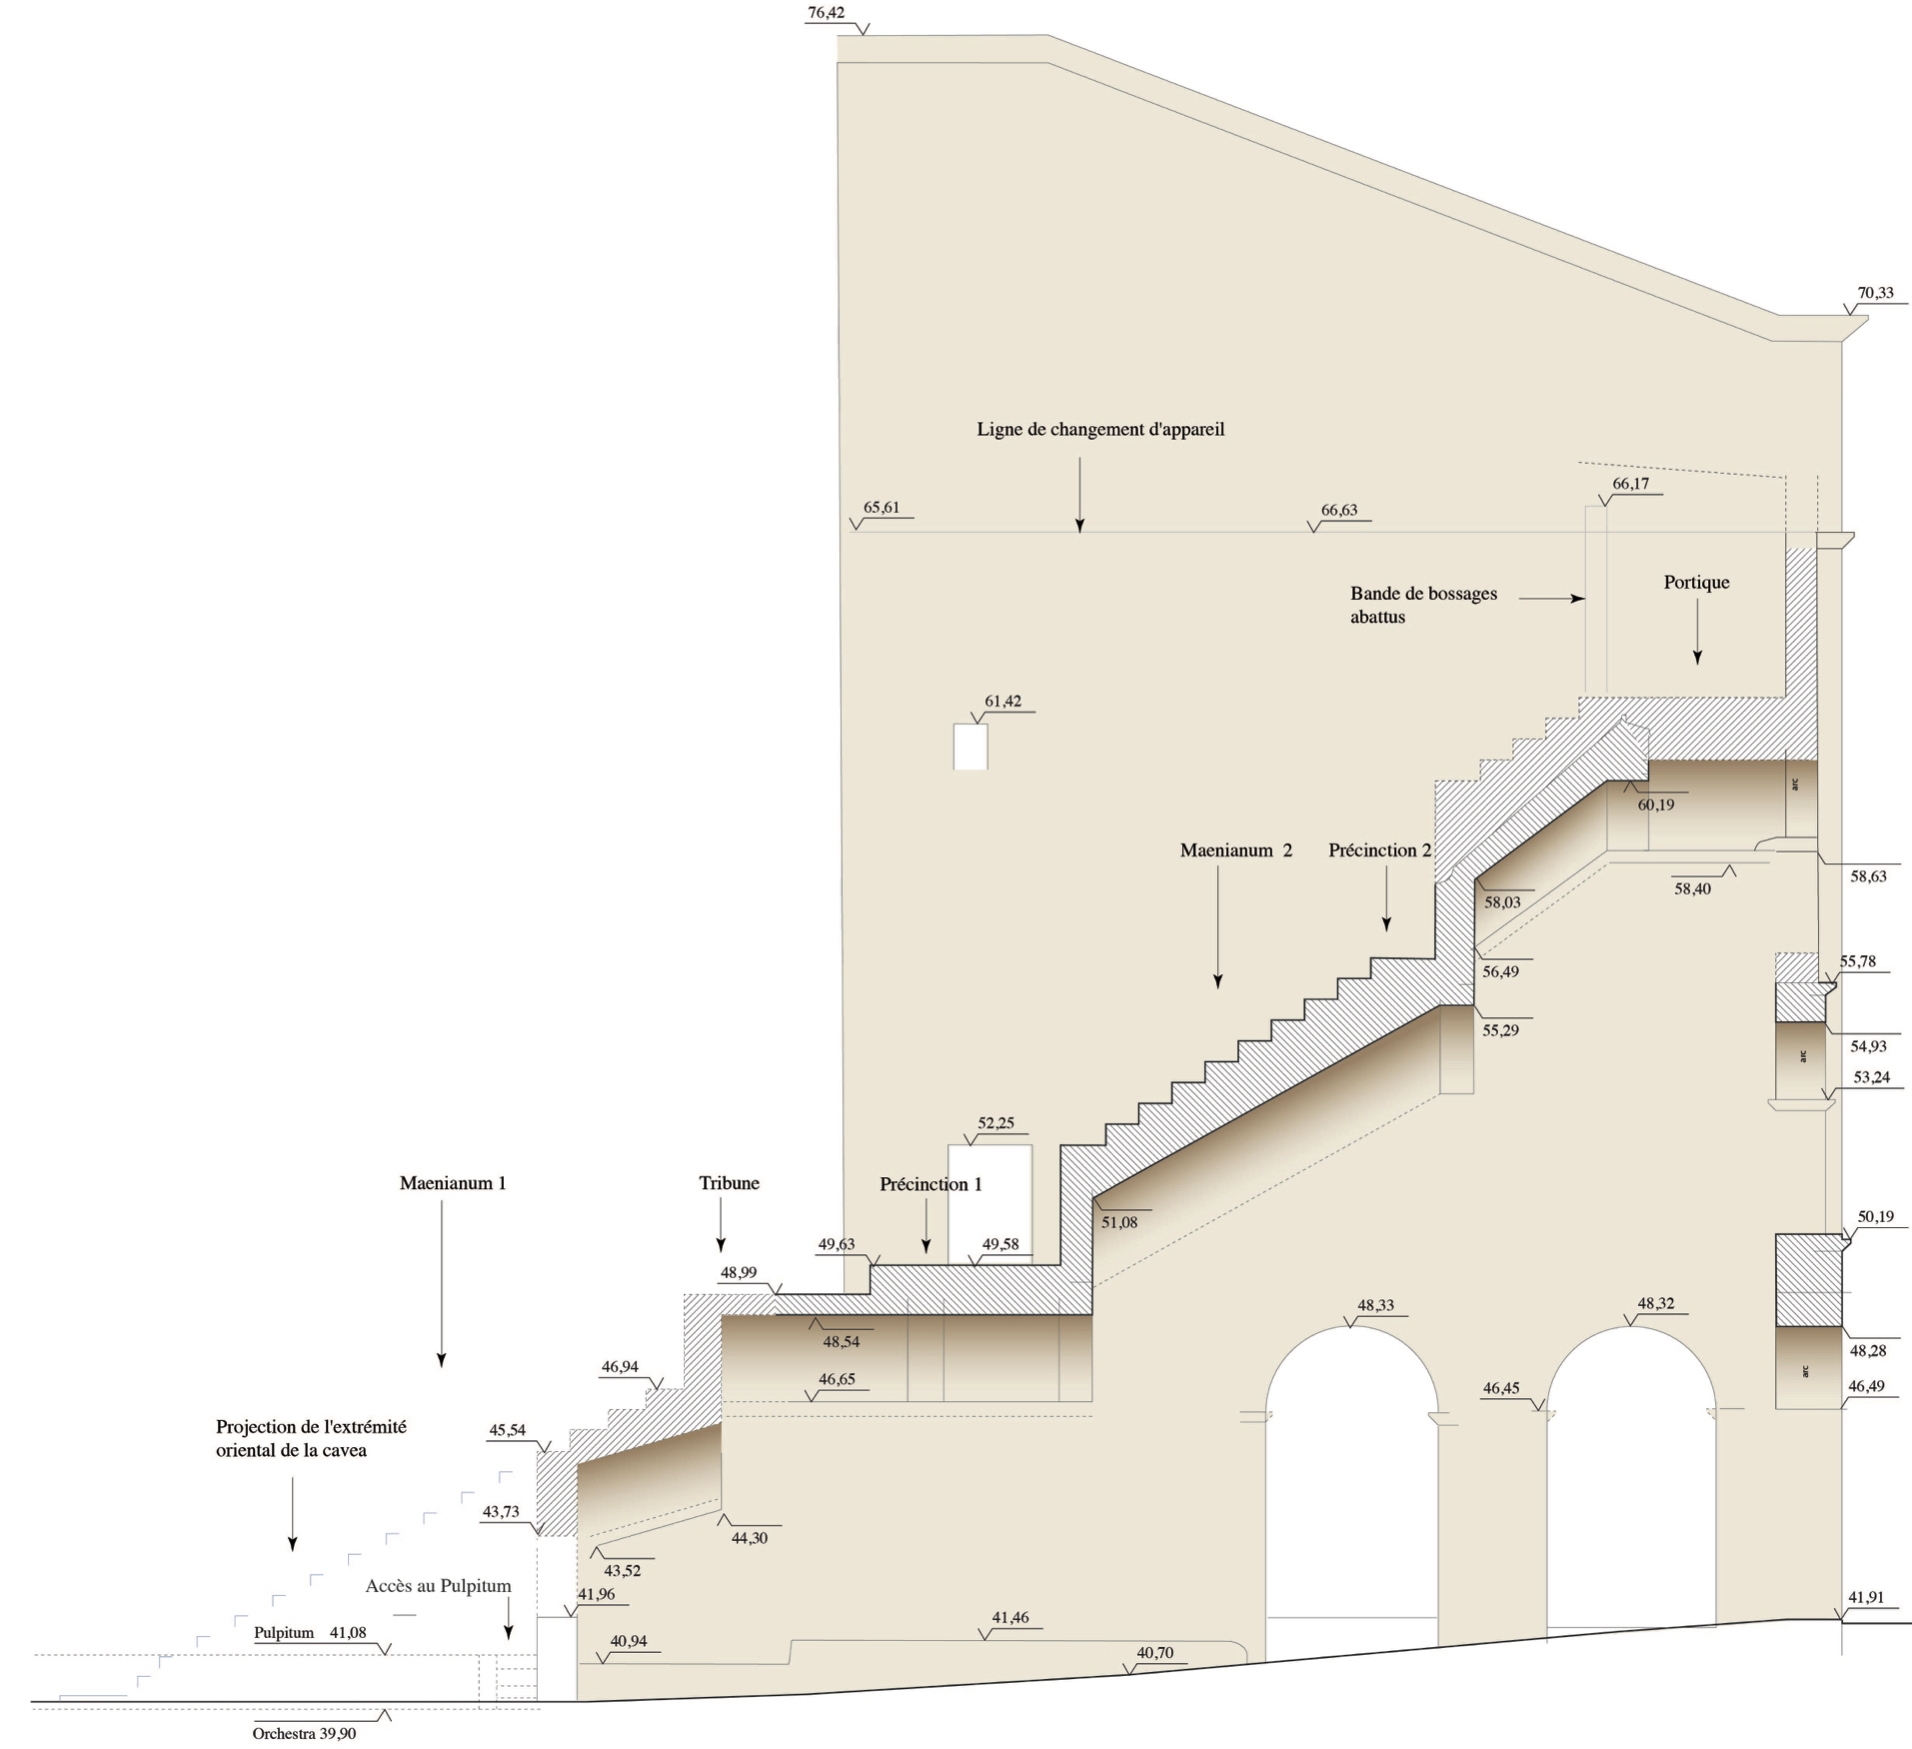
\includegraphics[width=\linewidth]{images/aditusOriental}
		\caption[Coupe sur l'\gls{aditus} oriental.]{Coupe sur l'\gls{aditus} oriental \cite[Pl. XLIX]{orangePl}.}
		\label{aditusOriental}
\end{figureth}

\begin{figureth}
	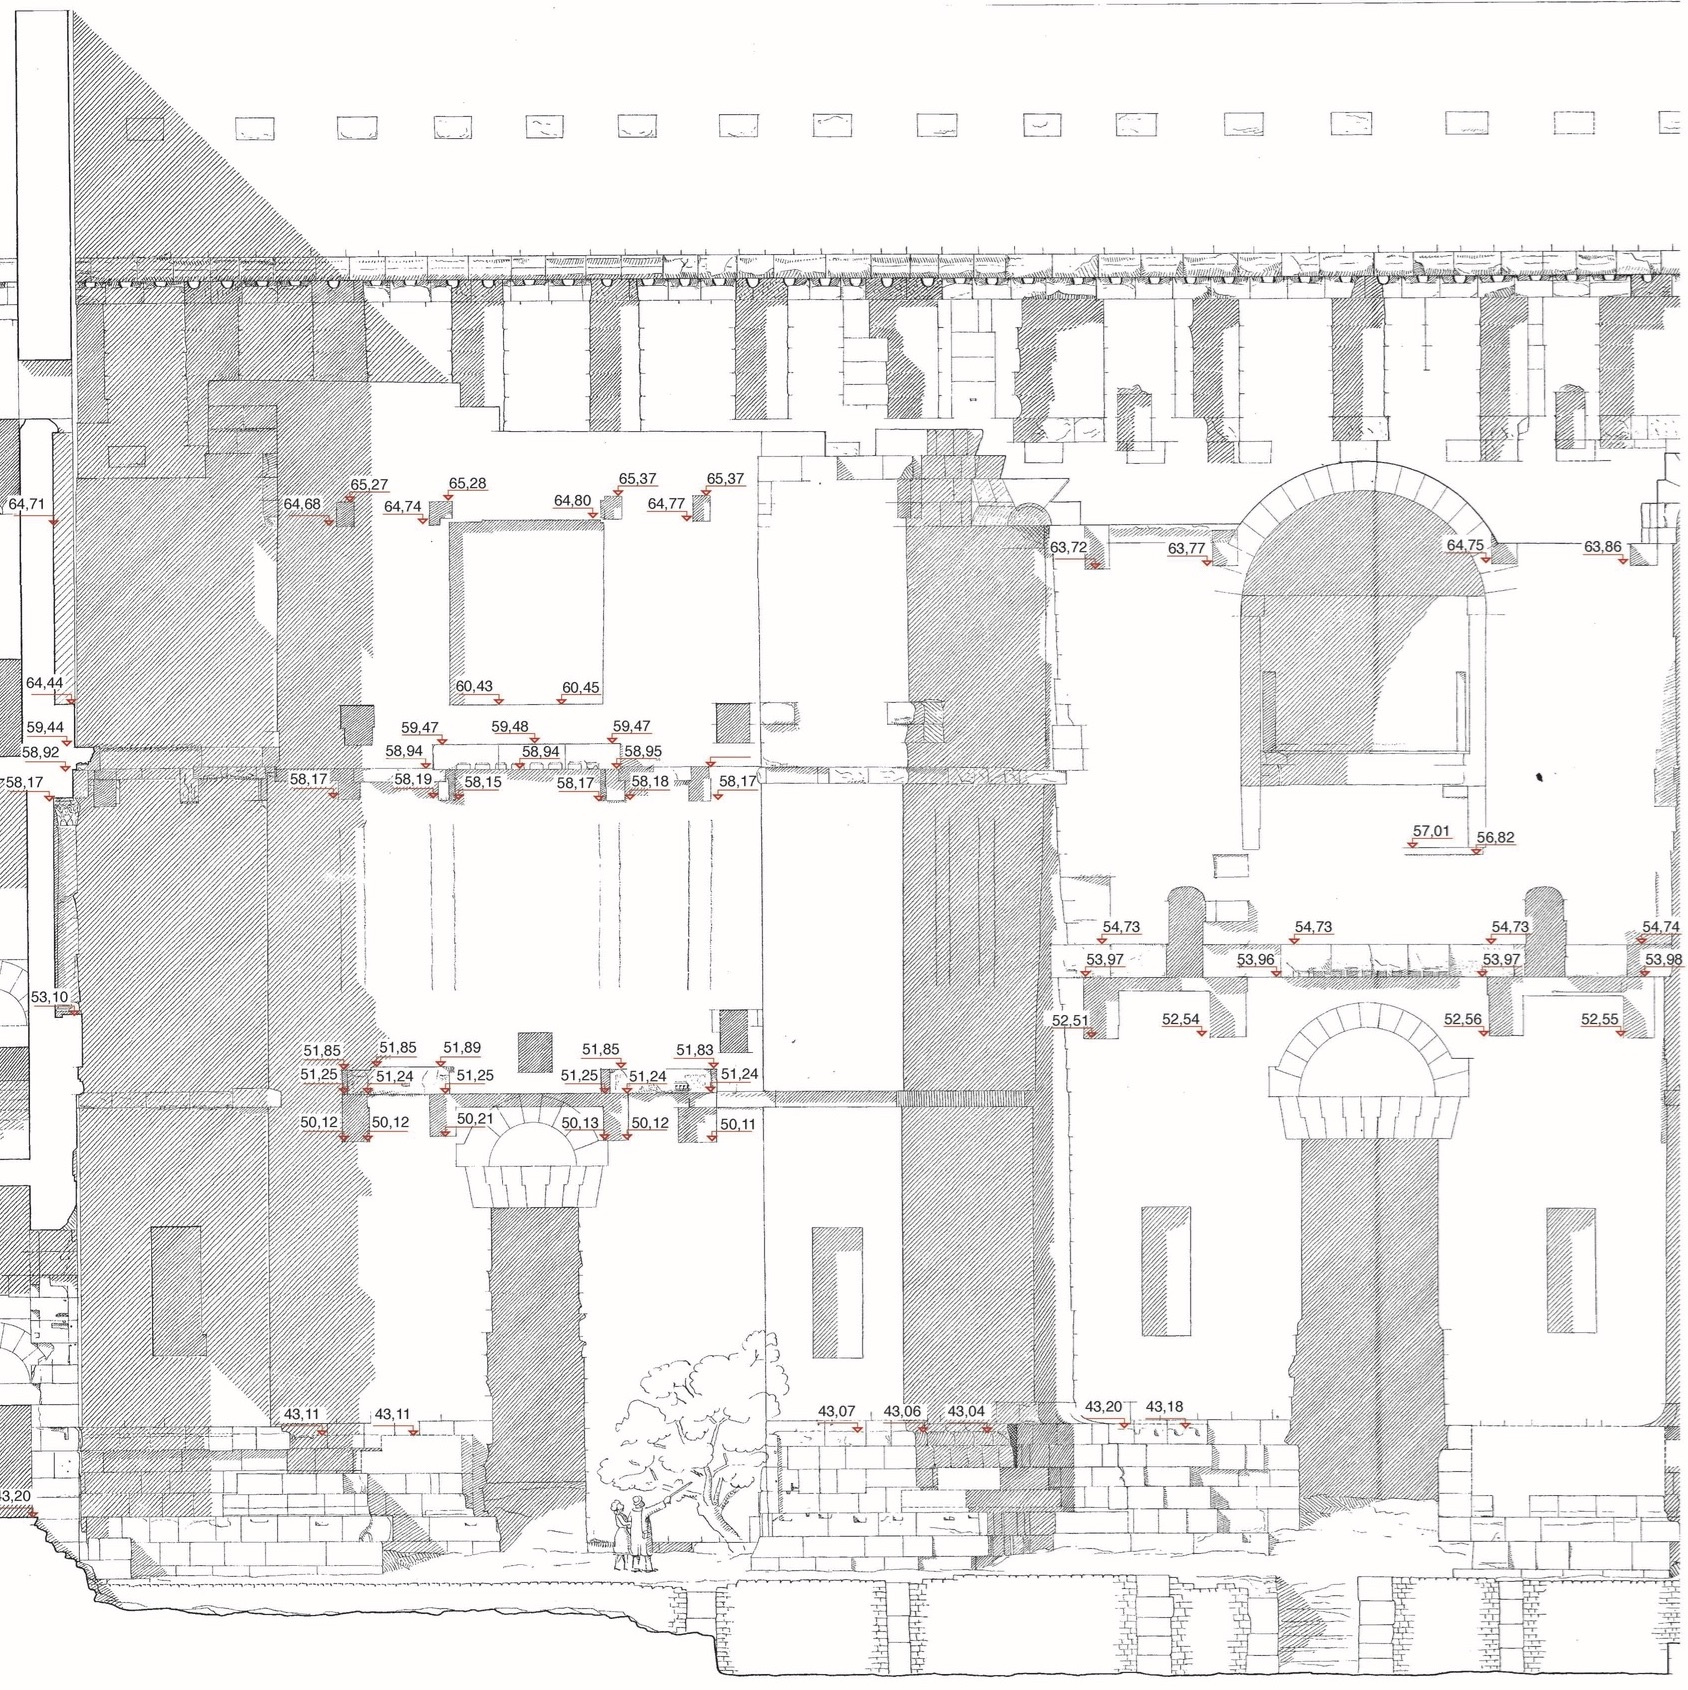
\includegraphics[width=\linewidth]{images/frontdescene}
	\caption[Elévation du front de scène.]{Elévation de la partie occidentale du front de scène nivelé \cite[Pl. XXIX]{orangePl}.}
	\label{frontdescene} 
\end{figureth}
	
\begin{figureth}
	\includegraphics[height=0.8\paperheight]{images/retourOccidentalMur}
	\caption[Elévation du retour du mur de scèn.e]{Élévation du retour occidental du mur de scène \cite[Pl. XXVII]{orangePl}.}
	\label{retourmur} 
\end{figureth}

\begin{figureth}
	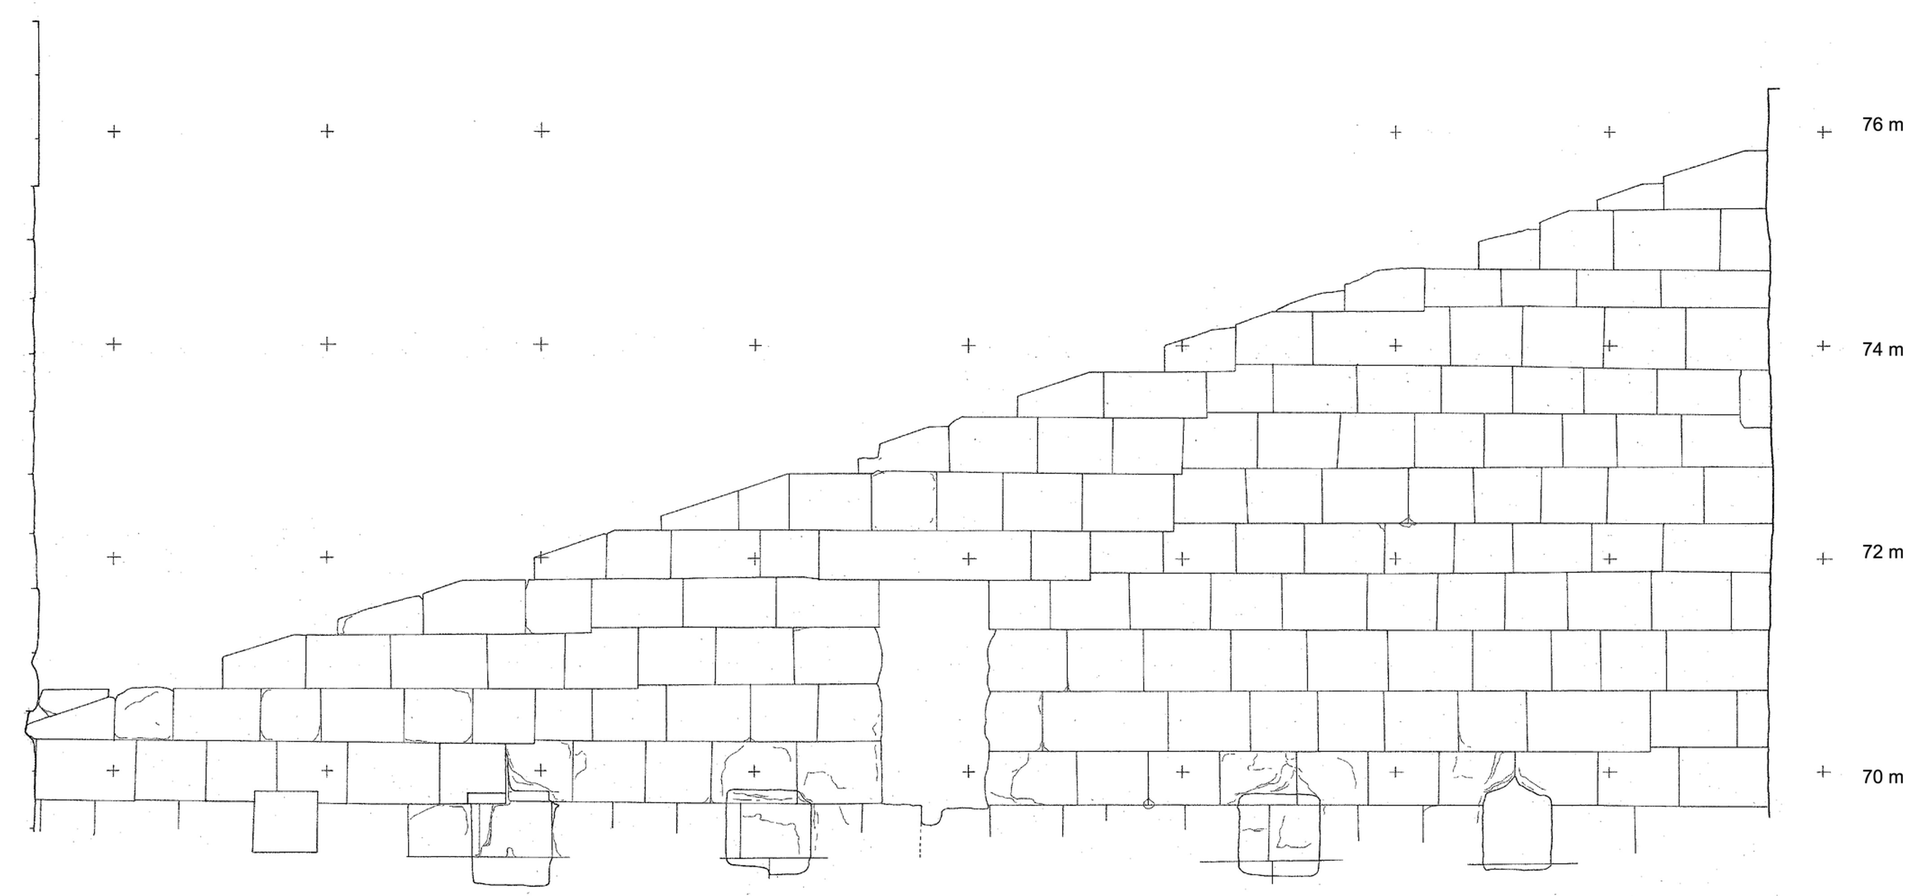
\includegraphics[width=\linewidth]{images/grenierOcci}
	\caption[Elévation de la partie sommitale de la basilique occidentale.]{Elévation de la partie sommitale de la basilique occidentale \cite[Pl. XLVI]{orangePl}.}
	\label{grenier} 
\end{figureth}

\begin{figureth}
	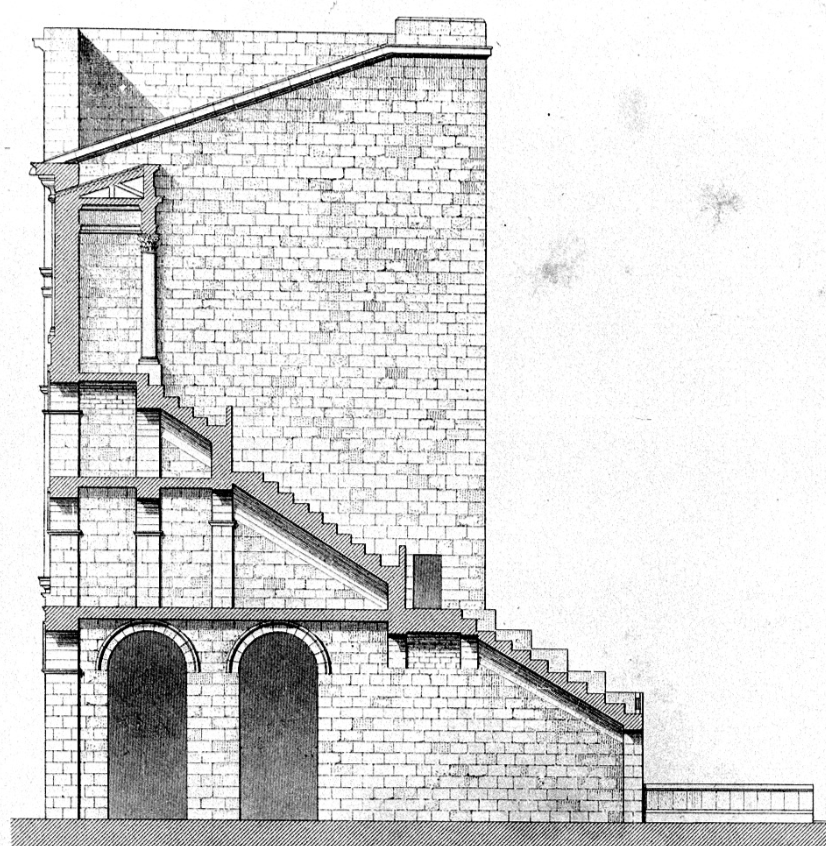
\includegraphics[width=\linewidth]{images/colonneCaristie}
	\caption[Coupe de l'\gls{aditus} occidental par A.Caristie - 1856.]{Coupe de l'\gls{aditus} occidental par A.Caristie - 1856 \cite[Pl. VI]{orangePl}.}
	\label{colonneCaristie} 
\end{figureth}

\begin{figureth}
	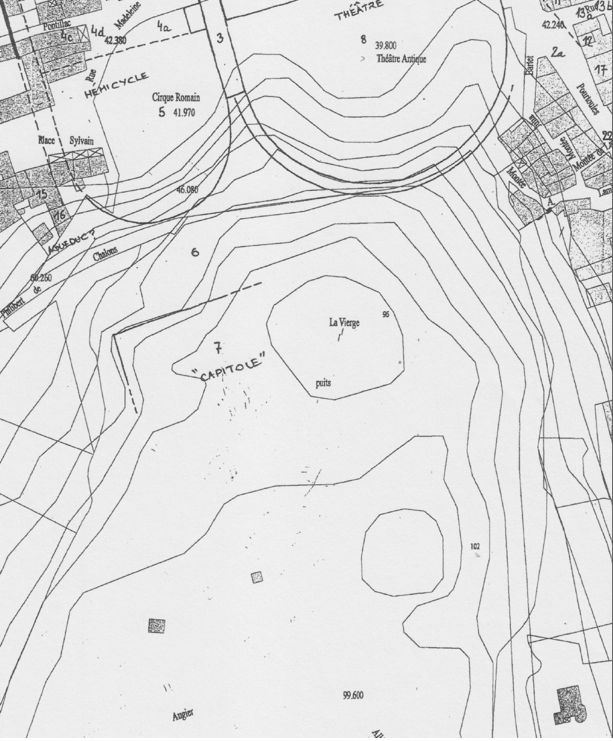
\includegraphics[width=\linewidth]{images/colline}
	\caption[Plan topographique de la colline Saint-Eutrope.]{Plan topographique de la colline Saint-Eutrope \cite[p.11]{orangeTxt}.}
	\label{colline} 
\end{figureth}	

\begin{figureth}
	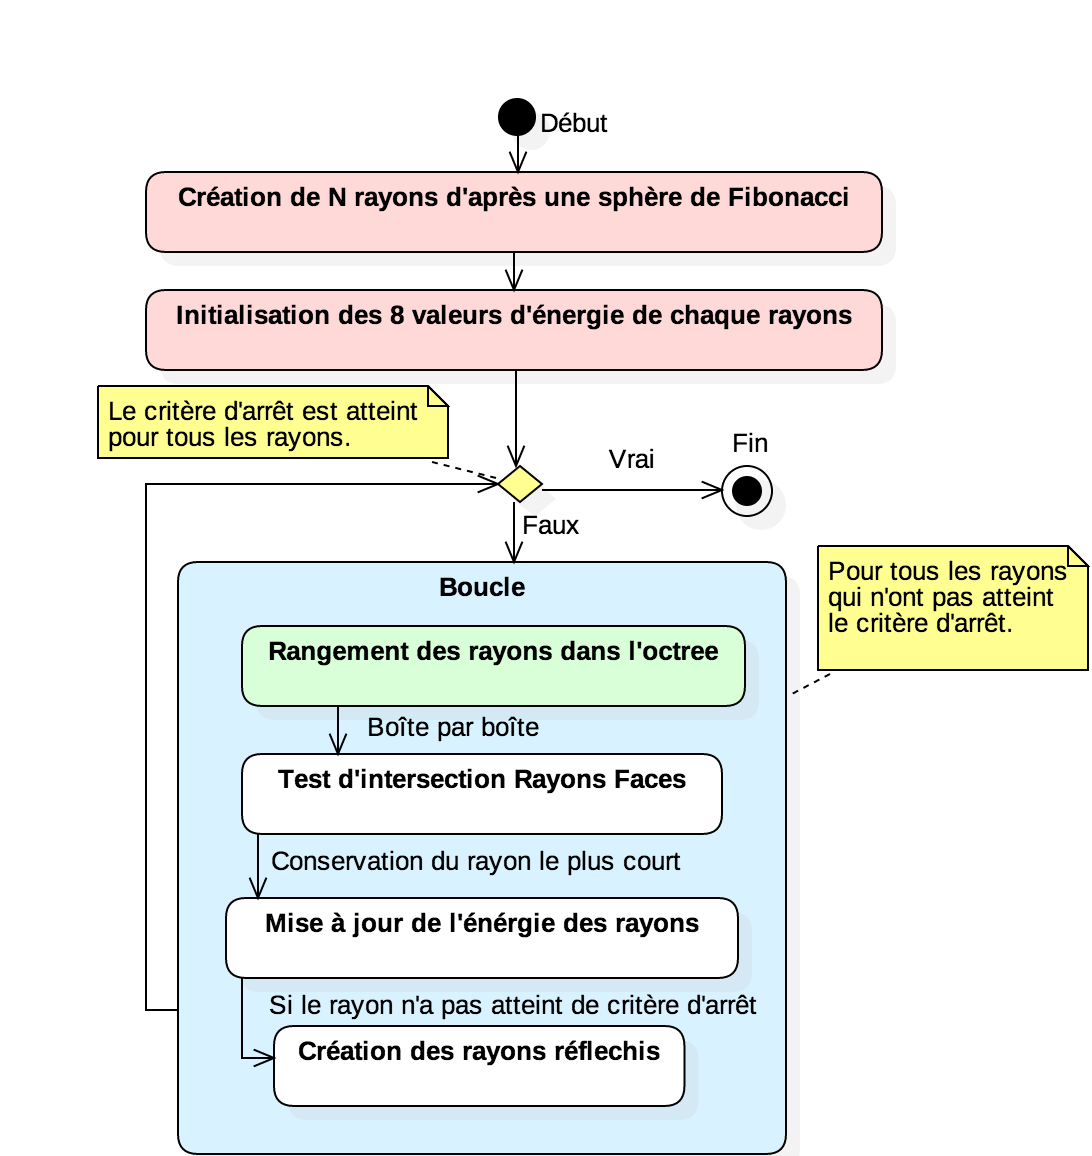
\includegraphics[width=0.9\linewidth]{images/DiagRay2}
	\caption{Diagramme d'activité résumant le processus de création des rayons avec \gls{octree}.}
	\label{DiagRay2}
\end{figureth}

\section*{Tableaux annexes}

\begin{table}[!h]
\footnotesize
 \begin{tabular}{| *{9}{c|}} 
 \hline 
 Récepteur & [x ; y ; z] (m)  & \gls{EDT} (ms) & \gls{T30} (ms) & \gls{spl} (dB) & \gls{C80} (dB) & \gls{D50} (\%) & \gls{Ts} (ms) \\ %& \gls{LF80} (dB) \\ 
 \hline 
 \hline 
1  & [0 ; -10.67 ; 41.44] &1310  &2861   &-29  &2.98  &60.14  &81 \\%listener12
 \hline 
 Réf    &[0 ; -16.5 ; 43.9] &1501  &2966   &-32  &3.65  &58.48  &81 \\%listenerREF
 \hline 
 2  & [0 ; -28.23 ; 50.02] &2163  &3690   &-35  &1.11  &42.03  &129 \\ %listener11
 \hline 
 3  &  [0 ; -37.86 ; 55.92] &2023  &4285   &-37  &0.31  &37.48  &133 \\ %listener10
 \hline 
 4  &  [0 ; -44.36 ; 62.06] &2439  &4335   &-37  &-0.72  &34.69  &155 \\%listener9
 \hline 
 \hline
 5  &   [-8.74 ; -6.12 ; 41.44] &1539  &2788   &-28  &3.81  &62.14  &80 \\%listener5
 \hline 
 6  &  [-13.51 ; -9.46 ; 43.86] &1479  &3383   &-31  &4.78  &64.28  &79 \\%listener4
  \hline 
  7 &   [-23.12 ; -16.19 ; 50.02] &2130  &3892   &-34  &3.22  &52.99  &119 \\ %listener6
 \hline 
 8  &  [-31.02 ; -21.72 ; 55.92] &2342  &3916   &-37  &1.89  &52.76  &140 \\ %listener7
 \hline 
 9  & [-36.34 ; -25.44 ; 62.06] &2893  &4444   &-38  &0.17  &38.92  &177 \\ %listener8
 \hline 
 \hline
 10  &  [-28.23 ; 1.66 ; 50.02] &2650  &4507   &-33  &-0.32  &39.73  &168 \\ %listener3
 \hline 
11   & [-37.87 ; 1.66 ; 55.92] &3189  & 3951  &-37  & -1.24 &41.56  &205 \\%listener2
 \hline 
12   & [-44.36 ; 1.66 ; 62.06] &3611  & 4487  & -36 &-2.66  &31.9  & 256\\ %listener1
 \hline 
\end{tabular} 
 \caption{Facteurs perceptifs pour différents récepteurs sur la bande de fréquence de 500Hz pour 1~000~000 de rayons sans le toit.} 
 \label{tab_fac_listener_sansToit} 
 \end{table}
 
\section*{Article}
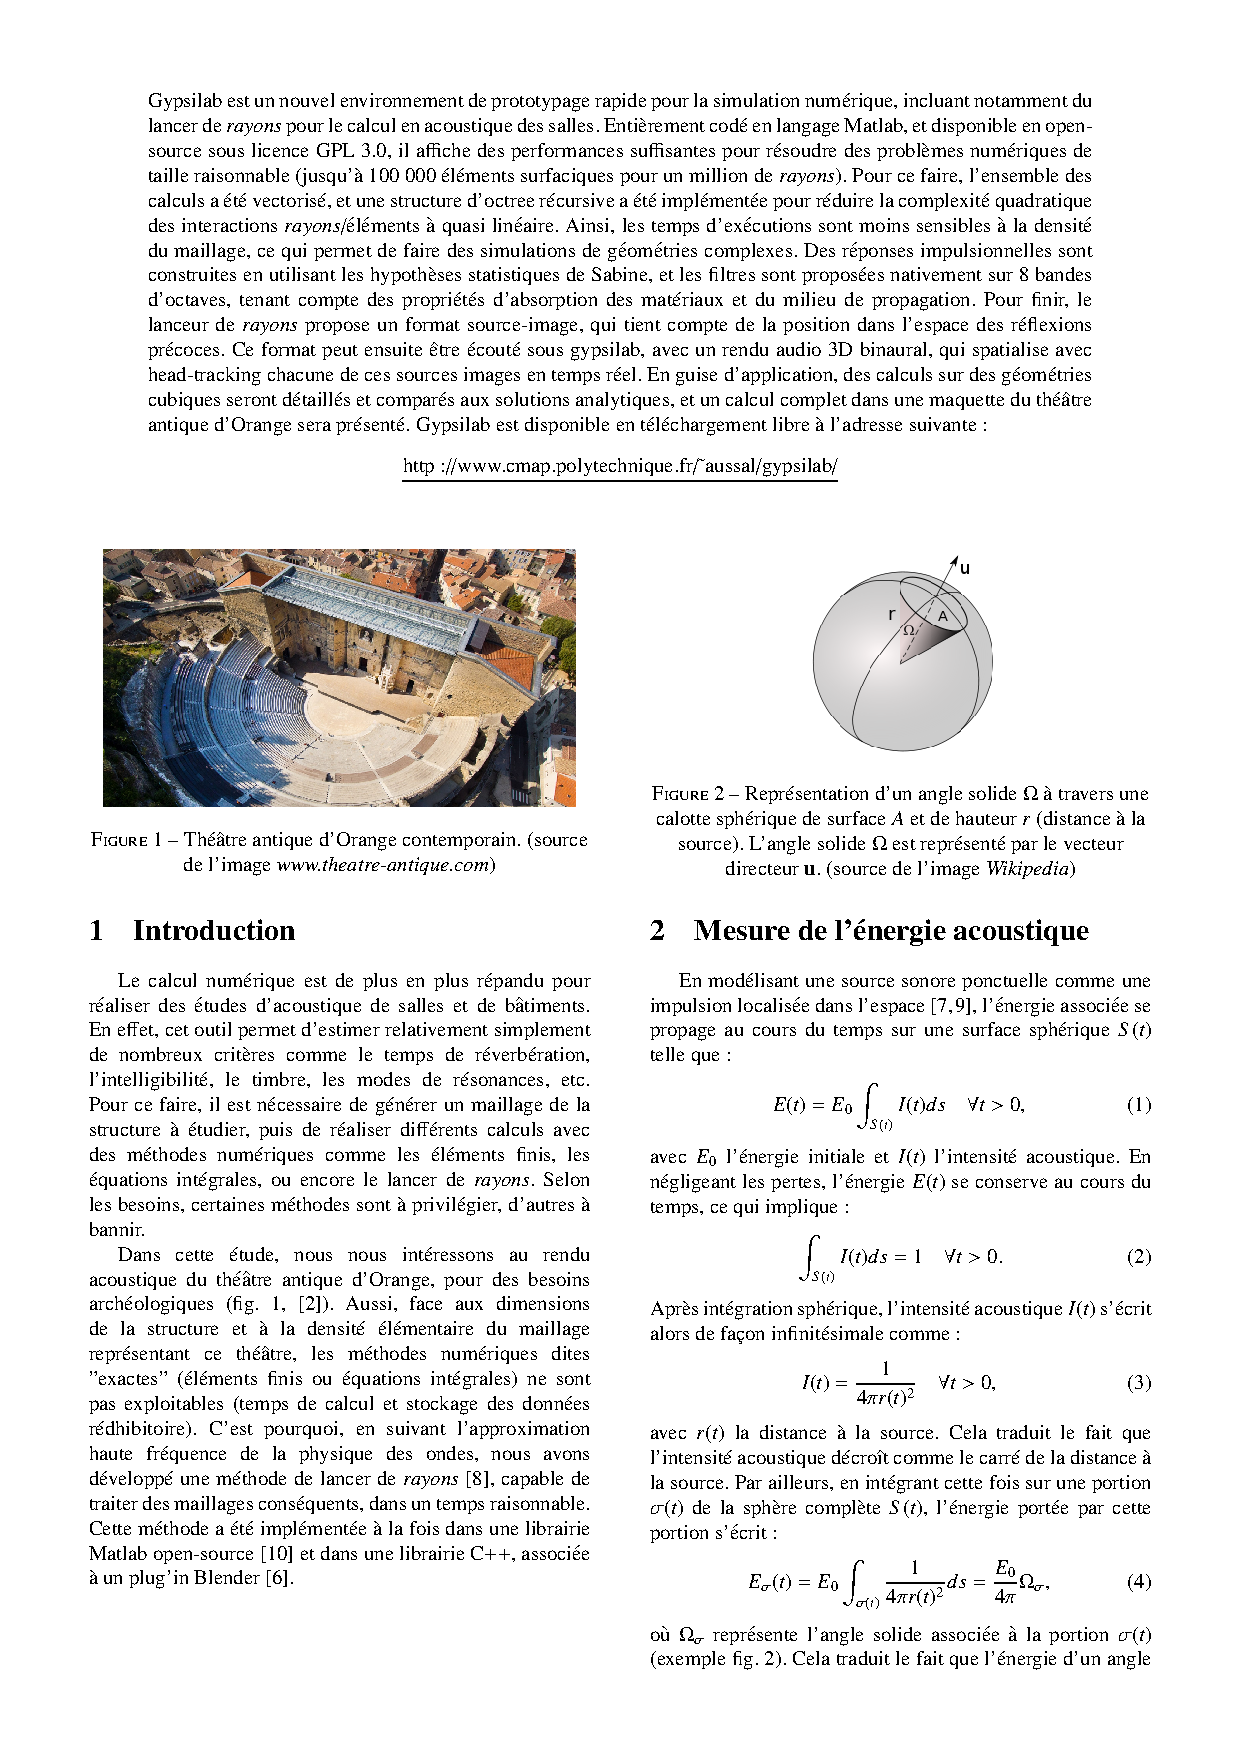
\includepdf[pages=1-6]{images/CFA2018_Aussal_Gueguen.pdf}

 \bibliographystyle{francaissc}
 \bibliography{Part1/Biblio}